

\tikzset{every picture/.style={line width=0.75pt}} %set default line width to 0.75pt        

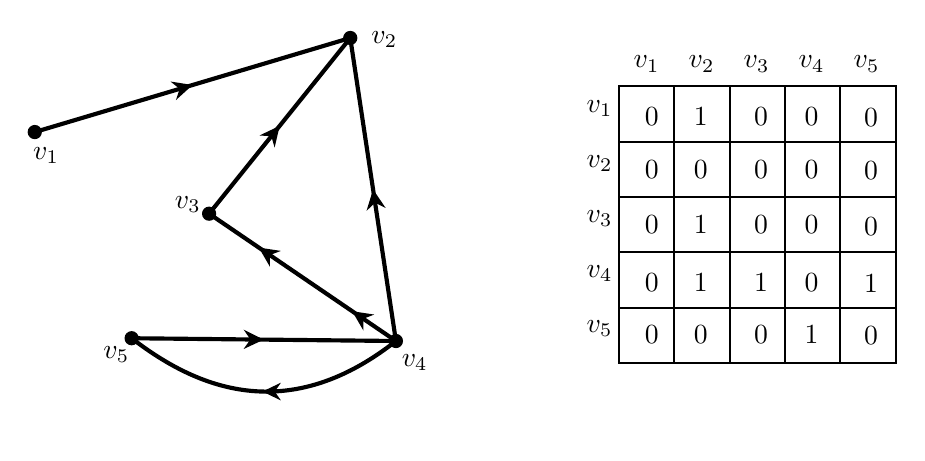
\begin{tikzpicture}[x=0.5pt,y=0.5pt,yscale=-1,xscale=1]
%uncomment if require: \path (0,299); %set diagram left start at 0, and has height of 299

%Flowchart: Connector [id:dp14554034773886415] 
\draw  [fill={rgb, 255:red, 0; green, 0; blue, 0 }  ,fill opacity=1 ] (25,96) .. controls (25,93.58) and (26.96,91.62) .. (29.38,91.62) .. controls (31.79,91.62) and (33.75,93.58) .. (33.75,96) .. controls (33.75,98.42) and (31.79,100.38) .. (29.38,100.38) .. controls (26.96,100.38) and (25,98.42) .. (25,96) -- cycle ;
%Flowchart: Connector [id:dp7796394659617965] 
\draw  [fill={rgb, 255:red, 0; green, 0; blue, 0 }  ,fill opacity=1 ] (253,28) .. controls (253,25.58) and (254.96,23.62) .. (257.38,23.62) .. controls (259.79,23.62) and (261.75,25.58) .. (261.75,28) .. controls (261.75,30.42) and (259.79,32.38) .. (257.38,32.38) .. controls (254.96,32.38) and (253,30.42) .. (253,28) -- cycle ;
%Flowchart: Connector [id:dp8410872532958124] 
\draw  [fill={rgb, 255:red, 0; green, 0; blue, 0 }  ,fill opacity=1 ] (286,247) .. controls (286,244.58) and (287.96,242.62) .. (290.38,242.62) .. controls (292.79,242.62) and (294.75,244.58) .. (294.75,247) .. controls (294.75,249.42) and (292.79,251.38) .. (290.38,251.38) .. controls (287.96,251.38) and (286,249.42) .. (286,247) -- cycle ;
%Flowchart: Connector [id:dp17196535593949425] 
\draw  [fill={rgb, 255:red, 0; green, 0; blue, 0 }  ,fill opacity=1 ] (95,245) .. controls (95,242.58) and (96.96,240.62) .. (99.38,240.62) .. controls (101.79,240.62) and (103.75,242.58) .. (103.75,245) .. controls (103.75,247.42) and (101.79,249.38) .. (99.38,249.38) .. controls (96.96,249.38) and (95,247.42) .. (95,245) -- cycle ;
%Straight Lines [id:da7073971572516686] 
\draw [color={rgb, 255:red, 0; green, 0; blue, 0 }  ,draw opacity=1 ][line width=1.5]    (29.38,96) -- (257.38,28) ;
\draw [shift={(143.38,62)}, rotate = 523.39] [fill={rgb, 255:red, 0; green, 0; blue, 0 }  ,fill opacity=1 ][line width=0.08]  [draw opacity=0] (14.56,-6.99) -- (0,0) -- (14.56,6.99) -- (9.67,0) -- cycle    ;
%Flowchart: Connector [id:dp6372189195472704] 
\draw  [fill={rgb, 255:red, 0; green, 0; blue, 0 }  ,fill opacity=1 ] (151,155) .. controls (151,152.58) and (152.96,150.62) .. (155.38,150.62) .. controls (157.79,150.62) and (159.75,152.58) .. (159.75,155) .. controls (159.75,157.42) and (157.79,159.38) .. (155.38,159.38) .. controls (152.96,159.38) and (151,157.42) .. (151,155) -- cycle ;
%Straight Lines [id:da6054846048754496] 
\draw [color={rgb, 255:red, 0; green, 0; blue, 0 }  ,draw opacity=1 ][line width=1.5]    (155.38,155) -- (257.38,28) ;
\draw [shift={(206.38,91.5)}, rotate = 488.77] [fill={rgb, 255:red, 0; green, 0; blue, 0 }  ,fill opacity=1 ][line width=0.08]  [draw opacity=0] (14.56,-6.99) -- (0,0) -- (14.56,6.99) -- (9.67,0) -- cycle    ;
%Straight Lines [id:da8238439208450634] 
\draw [color={rgb, 255:red, 0; green, 0; blue, 0 }  ,draw opacity=1 ][line width=1.5]    (99.38,245) -- (290.38,247) ;
\draw [shift={(194.88,246)}, rotate = 180.6] [fill={rgb, 255:red, 0; green, 0; blue, 0 }  ,fill opacity=1 ][line width=0.08]  [draw opacity=0] (14.56,-6.99) -- (0,0) -- (14.56,6.99) -- (9.67,0) -- cycle    ;
%Straight Lines [id:da4336320329770583] 
\draw [color={rgb, 255:red, 0; green, 0; blue, 0 }  ,draw opacity=1 ][line width=1.5]    (290.38,247) -- (257.38,28) ;
\draw [shift={(273.88,137.5)}, rotate = 441.43] [fill={rgb, 255:red, 0; green, 0; blue, 0 }  ,fill opacity=1 ][line width=0.08]  [draw opacity=0] (14.56,-6.99) -- (0,0) -- (14.56,6.99) -- (9.67,0) -- cycle    ;
%Straight Lines [id:da684522286123465] 
\draw [color={rgb, 255:red, 0; green, 0; blue, 0 }  ,draw opacity=1 ][line width=1.5]    (290.38,247) -- (227.18,203.93) -- (155.38,155) ;
\draw [shift={(258.78,225.47)}, rotate = 394.27] [fill={rgb, 255:red, 0; green, 0; blue, 0 }  ,fill opacity=1 ][line width=0.08]  [draw opacity=0] (14.56,-6.99) -- (0,0) -- (14.56,6.99) -- (9.67,0) -- cycle    ;
\draw [shift={(191.28,179.47)}, rotate = 394.27] [fill={rgb, 255:red, 0; green, 0; blue, 0 }  ,fill opacity=1 ][line width=0.08]  [draw opacity=0] (14.56,-6.99) -- (0,0) -- (14.56,6.99) -- (9.67,0) -- cycle    ;
%Curve Lines [id:da7415875935631565] 
\draw [line width=1.5]    (290.38,247) .. controls (208.63,311.52) and (141.63,277.52) .. (99.38,245) ;
\draw [shift={(193.9,283.53)}, rotate = 360.02] [fill={rgb, 255:red, 0; green, 0; blue, 0 }  ][line width=0.08]  [draw opacity=0] (13.4,-6.43) -- (0,0) -- (13.4,6.44) -- (8.9,0) -- cycle    ;
%Shape: Grid [id:dp07332615829400024] 
\draw  [draw opacity=0] (651.64,63) -- (451.64,63) -- (451.64,263) -- (651.64,263) -- cycle ; \draw   (611.64,63) -- (611.64,263)(571.64,63) -- (571.64,263)(531.64,63) -- (531.64,263)(491.64,63) -- (491.64,263) ; \draw   (651.64,103) -- (451.64,103)(651.64,143) -- (451.64,143)(651.64,183) -- (451.64,183)(651.64,223) -- (451.64,223) ; \draw   (651.64,63) -- (451.64,63) -- (451.64,263) -- (651.64,263) -- cycle ;

% Text Node
\draw (26,104.93) node [anchor=north west][inner sep=0.75pt]   [align=left] {$\displaystyle v_{1}$};
% Text Node
\draw (128.38,140.31) node [anchor=north west][inner sep=0.75pt]   [align=left] {$\displaystyle v_{3}$};
% Text Node
\draw (76.75,248.93) node [anchor=north west][inner sep=0.75pt]   [align=left] {$\displaystyle v_{5}$};
% Text Node
\draw (292.38,254.31) node [anchor=north west][inner sep=0.75pt]   [align=left] {$\displaystyle v_{4}$};
% Text Node
\draw (270.38,21.31) node [anchor=north west][inner sep=0.75pt]   [align=left] {$\displaystyle v_{2}$};
% Text Node
\draw (426,70.93) node [anchor=north west][inner sep=0.75pt]   [align=left] {$\displaystyle v_{1}$};
% Text Node
\draw (426,110.68) node [anchor=north west][inner sep=0.75pt]   [align=left] {$\displaystyle v_{2}$};
% Text Node
\draw (426,150.43) node [anchor=north west][inner sep=0.75pt]   [align=left] {$\displaystyle v_{3}$};
% Text Node
\draw (426,190.18) node [anchor=north west][inner sep=0.75pt]   [align=left] {$\displaystyle v_{4}$};
% Text Node
\draw (426,229.93) node [anchor=north west][inner sep=0.75pt]   [align=left] {$\displaystyle v_{5}$};
% Text Node
\draw (460,38.81) node [anchor=north west][inner sep=0.75pt]   [align=left] {$\displaystyle v_{1}$};
% Text Node
\draw (499.75,38.81) node [anchor=north west][inner sep=0.75pt]   [align=left] {$\displaystyle v_{2}$};
% Text Node
\draw (539.5,38.81) node [anchor=north west][inner sep=0.75pt]   [align=left] {$\displaystyle v_{3}$};
% Text Node
\draw (579.25,38.81) node [anchor=north west][inner sep=0.75pt]   [align=left] {$\displaystyle v_{4}$};
% Text Node
\draw (619,38.81) node [anchor=north west][inner sep=0.75pt]   [align=left] {$\displaystyle v_{5}$};
% Text Node
\draw (503.5,75.93) node [anchor=north west][inner sep=0.75pt]   [align=left] {$\displaystyle 1$};
% Text Node
\draw (503.5,195.93) node [anchor=north west][inner sep=0.75pt]   [align=left] {$\displaystyle 1$};
% Text Node
\draw (503.5,154.43) node [anchor=north west][inner sep=0.75pt]   [align=left] {$\displaystyle 1$};
% Text Node
\draw (547,195.93) node [anchor=north west][inner sep=0.75pt]   [align=left] {$\displaystyle 1$};
% Text Node
\draw (626.5,196.93) node [anchor=north west][inner sep=0.75pt]   [align=left] {$\displaystyle 1$};
% Text Node
\draw (583.5,233.43) node [anchor=north west][inner sep=0.75pt]   [align=left] {$\displaystyle 1$};
% Text Node
\draw (468,75.93) node [anchor=north west][inner sep=0.75pt]   [align=left] {$\displaystyle 0$};
% Text Node
\draw (626.5,115.43) node [anchor=north west][inner sep=0.75pt]   [align=left] {$\displaystyle 0$};
% Text Node
\draw (583.5,114.43) node [anchor=north west][inner sep=0.75pt]   [align=left] {$\displaystyle 0$};
% Text Node
\draw (547,75.93) node [anchor=north west][inner sep=0.75pt]   [align=left] {$\displaystyle 0$};
% Text Node
\draw (583.5,75.93) node [anchor=north west][inner sep=0.75pt]   [align=left] {$\displaystyle 0$};
% Text Node
\draw (626.5,76.93) node [anchor=north west][inner sep=0.75pt]   [align=left] {$\displaystyle 0$};
% Text Node
\draw (468,114.43) node [anchor=north west][inner sep=0.75pt]   [align=left] {$\displaystyle 0$};
% Text Node
\draw (503.5,114.43) node [anchor=north west][inner sep=0.75pt]   [align=left] {$\displaystyle 0$};
% Text Node
\draw (547,114.43) node [anchor=north west][inner sep=0.75pt]   [align=left] {$\displaystyle 0$};
% Text Node
\draw (626.5,155.43) node [anchor=north west][inner sep=0.75pt]   [align=left] {$\displaystyle 0$};
% Text Node
\draw (583.5,154.43) node [anchor=north west][inner sep=0.75pt]   [align=left] {$\displaystyle 0$};
% Text Node
\draw (547,154.43) node [anchor=north west][inner sep=0.75pt]   [align=left] {$\displaystyle 0$};
% Text Node
\draw (547,233.43) node [anchor=north west][inner sep=0.75pt]   [align=left] {$\displaystyle 0$};
% Text Node
\draw (503.5,233.43) node [anchor=north west][inner sep=0.75pt]   [align=left] {$\displaystyle 0$};
% Text Node
\draw (468,233.43) node [anchor=north west][inner sep=0.75pt]   [align=left] {$\displaystyle 0$};
% Text Node
\draw (468,154.43) node [anchor=north west][inner sep=0.75pt]   [align=left] {$\displaystyle 0$};
% Text Node
\draw (468,195.93) node [anchor=north west][inner sep=0.75pt]   [align=left] {$\displaystyle 0$};
% Text Node
\draw (583.5,195.93) node [anchor=north west][inner sep=0.75pt]   [align=left] {$\displaystyle 0$};
% Text Node
\draw (626.5,234.43) node [anchor=north west][inner sep=0.75pt]   [align=left] {$\displaystyle 0$};


\end{tikzpicture}

